\vspace{0.5cm}

\section*{Descripción e Idea}

\noindent Como inspiración para este proyecto se tomó el articulo (1), en este se toman regiones de formación estelar. La idea es utilizar el método de \textit{conteo de cajas} (Box Counting Method) para determinar la dimensión Hausdorff-Besicovitch (o dimensión fractal) de diversos paises, en concreto islas.  Y, con ello realizar un análisis respecto al número de cajas y tamaño de las mismas en los diferentes países al encontrar dicha dimensión por medio de un ajuste lineal.



\section*{Procedimiento/Trabajo a Realizar}

\noindent Investigar sobre el método de conteo de cajas, el trato de la imagen a simplemente su contorno e implementación del método, esto se pretende hacer con \textit{Mathematica} o \textit{Python} ya que estos lenguajes proveen formas de tratar con imagenes y luego utilizar estos mismos lenguajes o bien \textit{Gnuplot} para realizar las gráficas y los respectivos ajustes.





\section*{Visualización}



\begin{multicols}{2}


En el artículo se proporciona una imagen del hubble la cual se convierte y se trabaja con ella de la siguiente forma:

\begin{figure}[H]
	\centering
	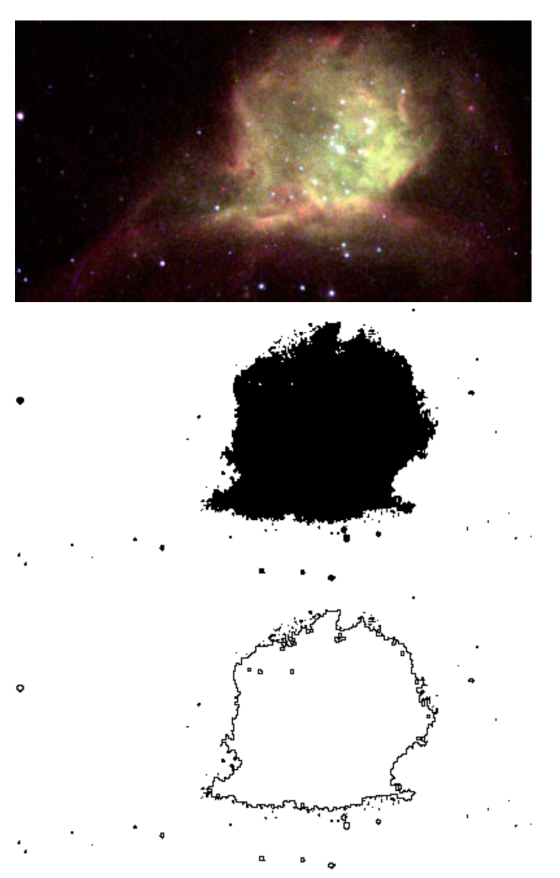
\includegraphics[scale=0.2]{./img/coso.png}
	\caption{Imagen tomada de (1), figura 2, p4.}
\end{figure}

\columnbreak

Con \textit{Mathematica} se puede generar el contorno de un país con la siguiente función \texttt{GeoGraphics[{GeoStyling["OutlineMap"], Polygon[Entity["Country", "Germany"]]}, GeoBackground -$>$ None]}, también con \textit{Python} se puede análizar y trabajar con imagenes utilizando la librería \texttt{OpenCV}.



\begin{figure}[H]
	\centering
	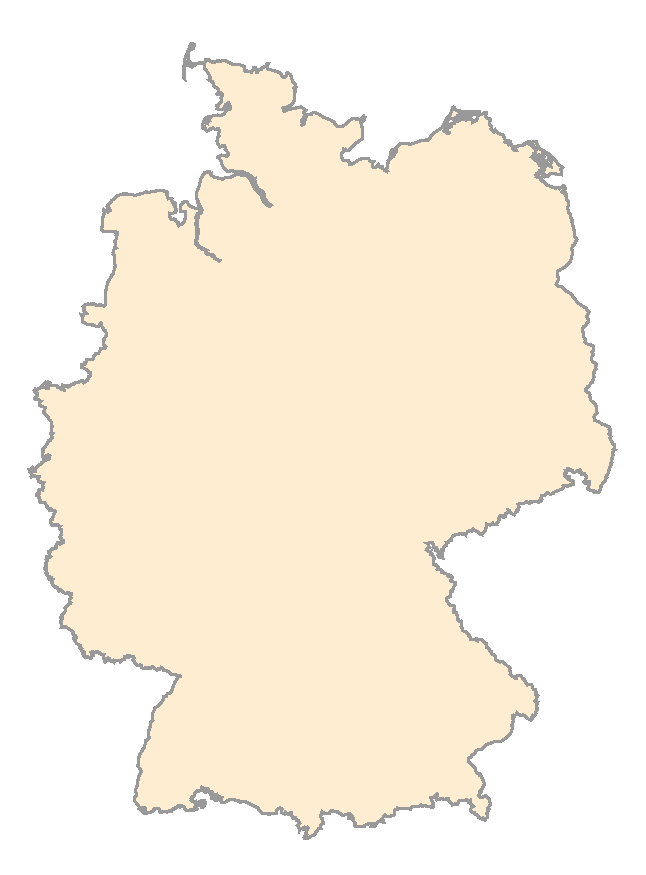
\includegraphics[scale=0.25]{./img/germany.pdf}
	\caption{Contorno de Alemania generado en \textit{Mathematica}.}
\end{figure}


\end{multicols}



%%%%%%%%%%%%%%%%%%%5


























%%%%%%%%%%%%%%%%%%%%%%%%5